%=================================================================

\section{Introduction}\label{sec-intro}

\subsection{Problem Statement}


After a month of making scientific observations 
and taking careful measurements, 
can determined that 900 ghouls, ghosts, and goblins
like the ~\cref{fig:animal} shows .
There are train data and test data,
through the train data to find the relationship
between the attributes and species.
Then identify 371 of the ghastly creatures


\begin{figure}[htbp]
	\centering
	\label{fig:animal}
	%\graphicspath{figures}
	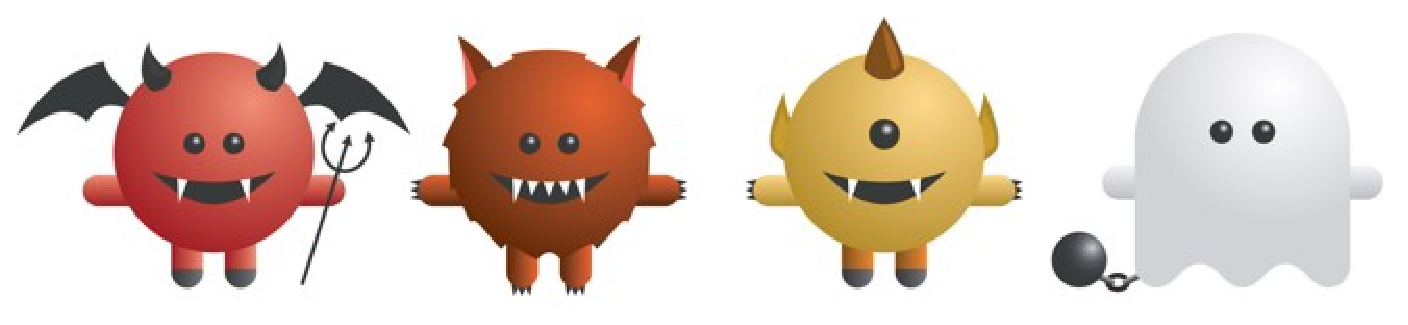
\includegraphics[scale=0.3]{figures/bar.eps}
	\caption{The Picture of Ghastly}
\end{figure}


\subsection{Data List}


There are bone length measurements, 
severity of rot, extent of soullessness, 
and other characteristics of the intruders,
the fllowings are the  
name and meaning of attributes


\begin{description}
	\item[id] id of the creature
	\item[bone_length] average length of bone in the creature, normalized between 0 and 1
	\item[rotting_flesh] percentage of rotting flesh in the creature
	\item[hair_length] average hair length, normalized between 0 and 1
	\item[has_soul] percentage of soul in the creature
	\item[Color] dominant color of the creature: 'white','black','clear','blue','green','blood'
	\item[type] target variable: 'Ghost', 'Goblin', and 'Ghoul'
\end{description}


\subsection{Problem Analysis}

\subsubsection{Train Data and Test Data}


Because this game is over, 
it can't submit the predictive values for testing. 
So divide the train data into train data and test data, 
and the ratio between the two is 8:2. 
And the data is small, 
so use ten-fold cross-validation 
to train the data.


\subsubsection{Problem Possible Solutions}


There are many machine learning algorithms 
can solve the three classification problem,
such as ensemble algorithms,
decision tree algorithm and so on.
Use CV to find the best parameters of the algorithms 
and then validate with testing data 


\subsubsection{Evaluation Methods}


Before experiment, determine the evaluation methods
to assess the model performance is very important,
usually it has two kinds of method for classification problem:

\begin{itemize}
	\item F1 Score/AUC
	\item Class Accuracy
\end{itemize} 


\section{Data exploration} \label{sec-data_exploration}

\subsection{Data Information}


The following table ~\cref{tbl:data information}
is the statistical result of the attribute values.
There are 4 numerical variables and 1 categorical. 
And no missing values.
Numerical columns are either normalized or show a percentage, 
so no need to scale them. 

\begin{table}[htbp]  \centering
	\caption{Data Information}
	\label{tbl:data information}
	\begin{tabular}{ccccccc}
		\hline
		% after \\: \hline or \cline{col1-col2} \cline{col3-col4} ...
		& bone_length & rotting_flesh & hair_length & has_soul & color & type\\
		\hline
		count & 371.0 & 371.0 & 371.0 & 371.0 & 371 & 371 \\
		unique & NaN & NaN & NaN & NaN & 6 & 3 \\
		top & NaN & NaN & NaN & NaN & white & Ghoul \\
		freq & NaN & NaN & NaN & NaN & 137 & 129\\
		mean & 0.434160 & 0.506848 & 0.529114 & 0.471392 & NaN & NaN \\
		std & 0.132833 & 0.146358 & 0.169902 & 0.176129 & NaN & NaN \\
		min & 0.061032 & 0.095687 & 0.134600 & 0.009402 & NaN & NaN \\
		25\% & 0.340006 & 0.414812 & 0.407428 & 0.348002 & NaN & NaN \\
		50\% & 0.43891 & 0.501552 & 0.538642 & 0.466372 & NaN & NaN\\
		75\% & 0.517223 & 0.603977 & 0.647244 & 0.600610 & NaN & NaN\\
		max &  0.817001 & 0.932466 & 1.000000 & 0.935721 & NaN & NaN\\
		\hline 
		%\bottomrule
	\end{tabular}
\end{table}


\subsection{Data Visualization}


Use EDA to plot the distribution of the data 
to can observate the data intuitively and
find the relation between the attribute values. 
For example boxplot can visually observe 
the distribution of numerical variables, 
scatterplot can show their distribution trends 
and whether there are outliers.
And for classification problems, 
the data is drawn according to 
the different colors of the Label, 
which is very helpful for 
the construction of the Feature.


\subsubsection{ Histogram}


The figure ~\cref{fig:his_1} 
shows the mean of the four numerical variables  
and the figure ~\cref{fig:his_2} 
is the number of different color 
about types of ghastly creatures.
It seems that all numerical features may be useful, 
but many colors are evenly distributes among the monsters. 
So they maybe not very useful for classification.


\begin{figure}[htbp]
	\centering
	\label{fig:his_1}
	%\graphicspath{{figures/}{mine/}}
	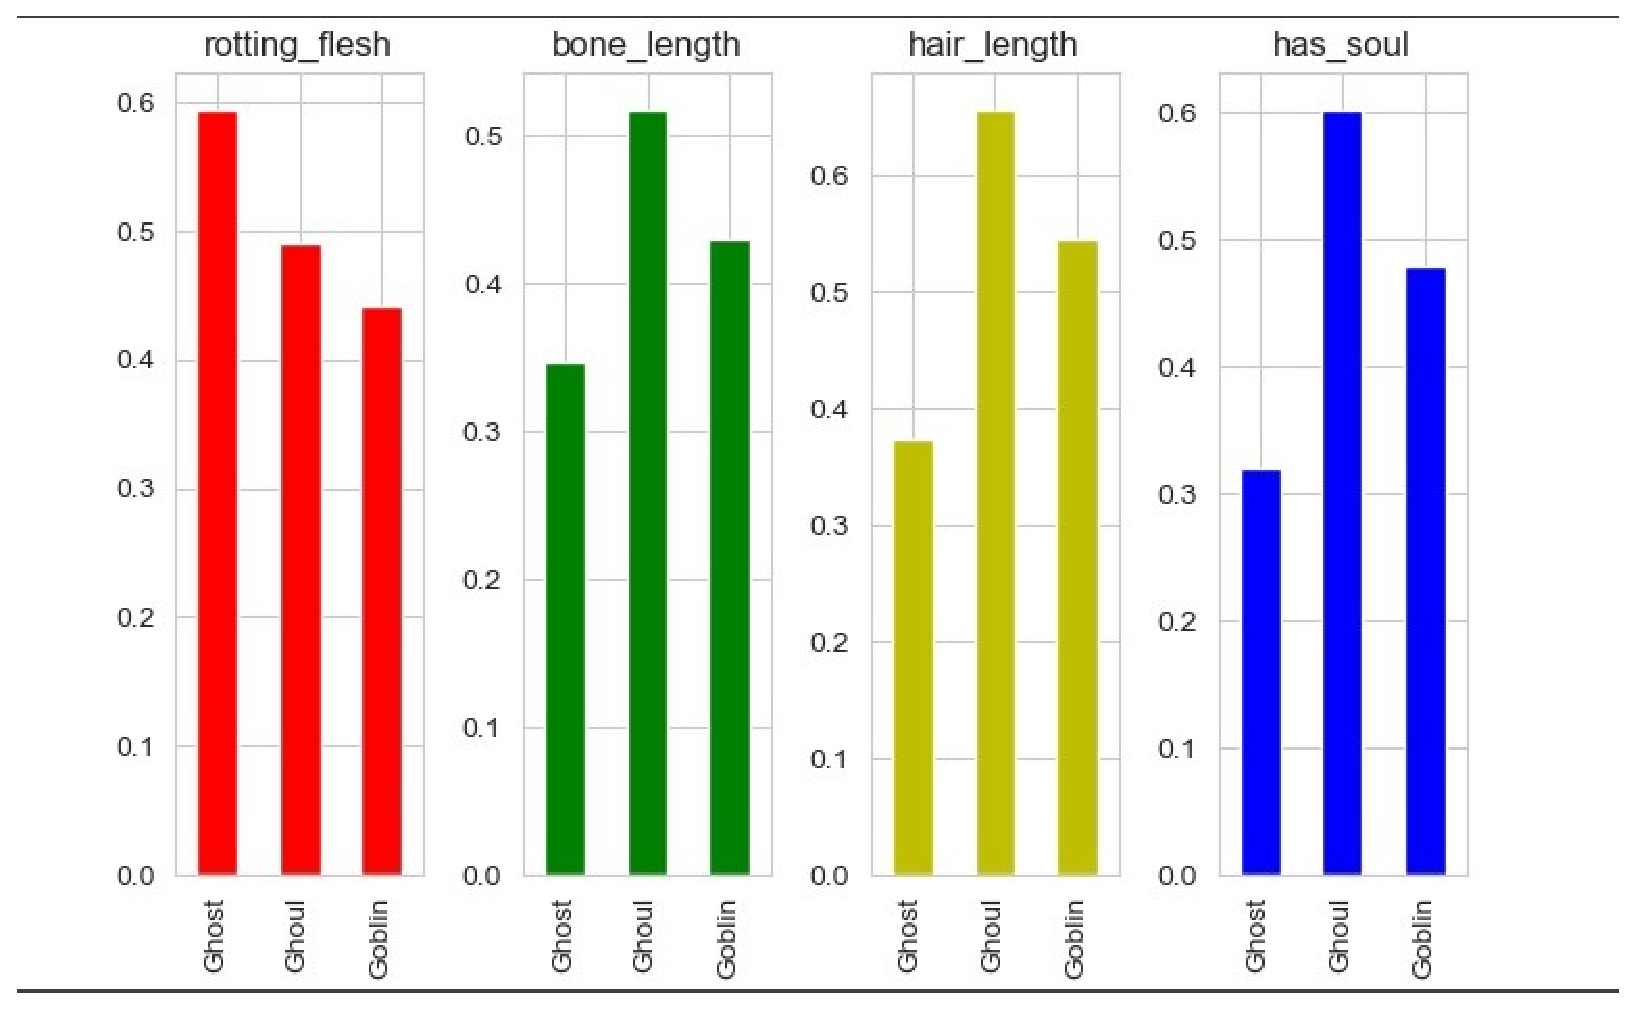
\includegraphics[scale=0.3]{figures/his_1.eps}
	\caption{The Mean of Four Numerical Variables}
\end{figure}


\begin{figure}[htbp]
	\centering
	\label{fig:his_2}
	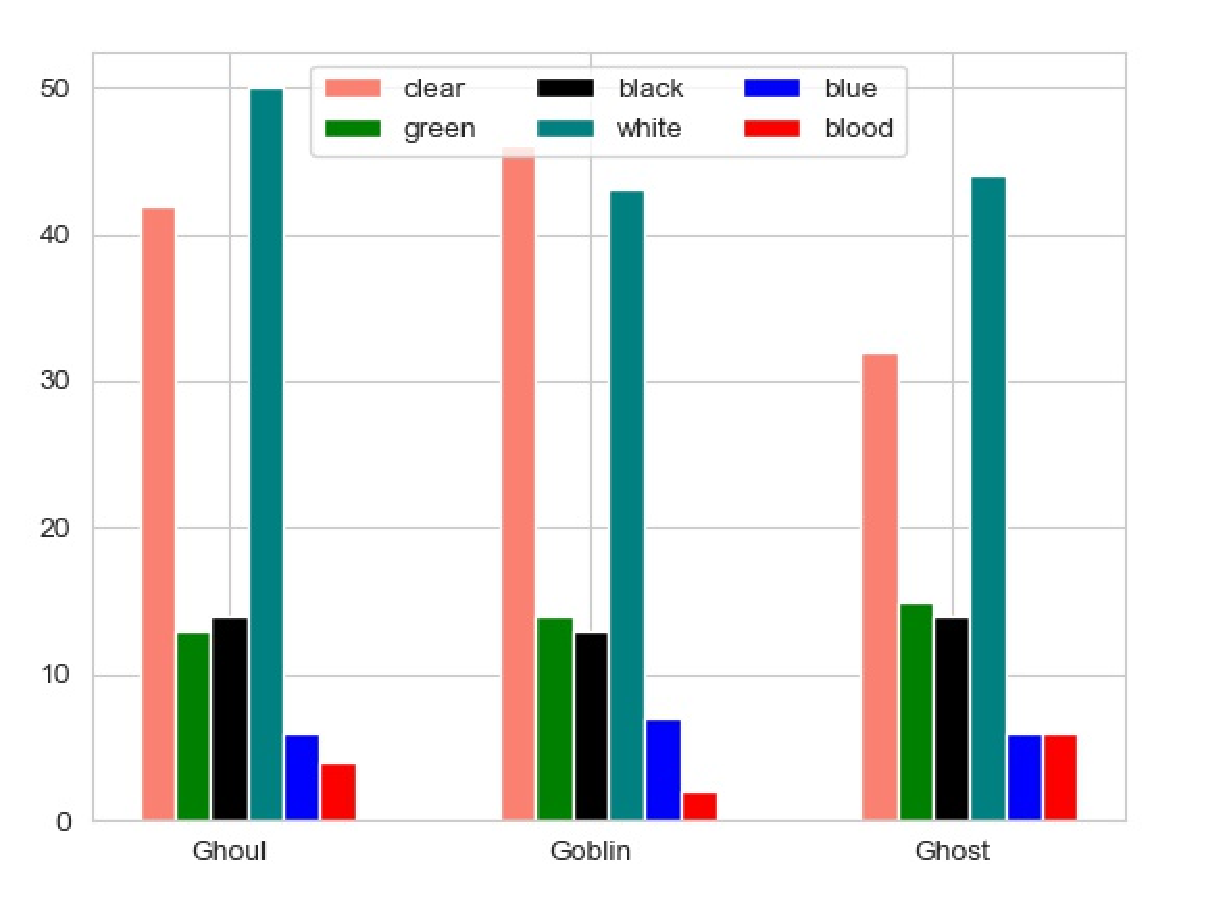
\includegraphics[scale=0.3]{figures/his_2.eps}
	\caption{Color distribution Grouped by Type}
\end{figure}


\subsubsection{Boxplot}

 
When analyzing the data, 
the boxplot can effectively 
help us identify the characteristics of the data: 
visually identify outliers in the dataset. 
Determine the data dispersion and 
bias of the data set. 
Through the figure ~\cref{fig:boxplot}, 
know that the two types of Ghost and Ghoul 
in the monster have higher discrimination 
on the four variables, 
while Goblin is in the middle position, 
which intersects with the other two types of features.
Guess that the predictive accuracy of Ghost and Ghoul 
will be better than Goblin.
And the outliers are very small,
which can be ignored.


\begin{figure}[htbp]
	\centering
	\label{fig:boxplot}
	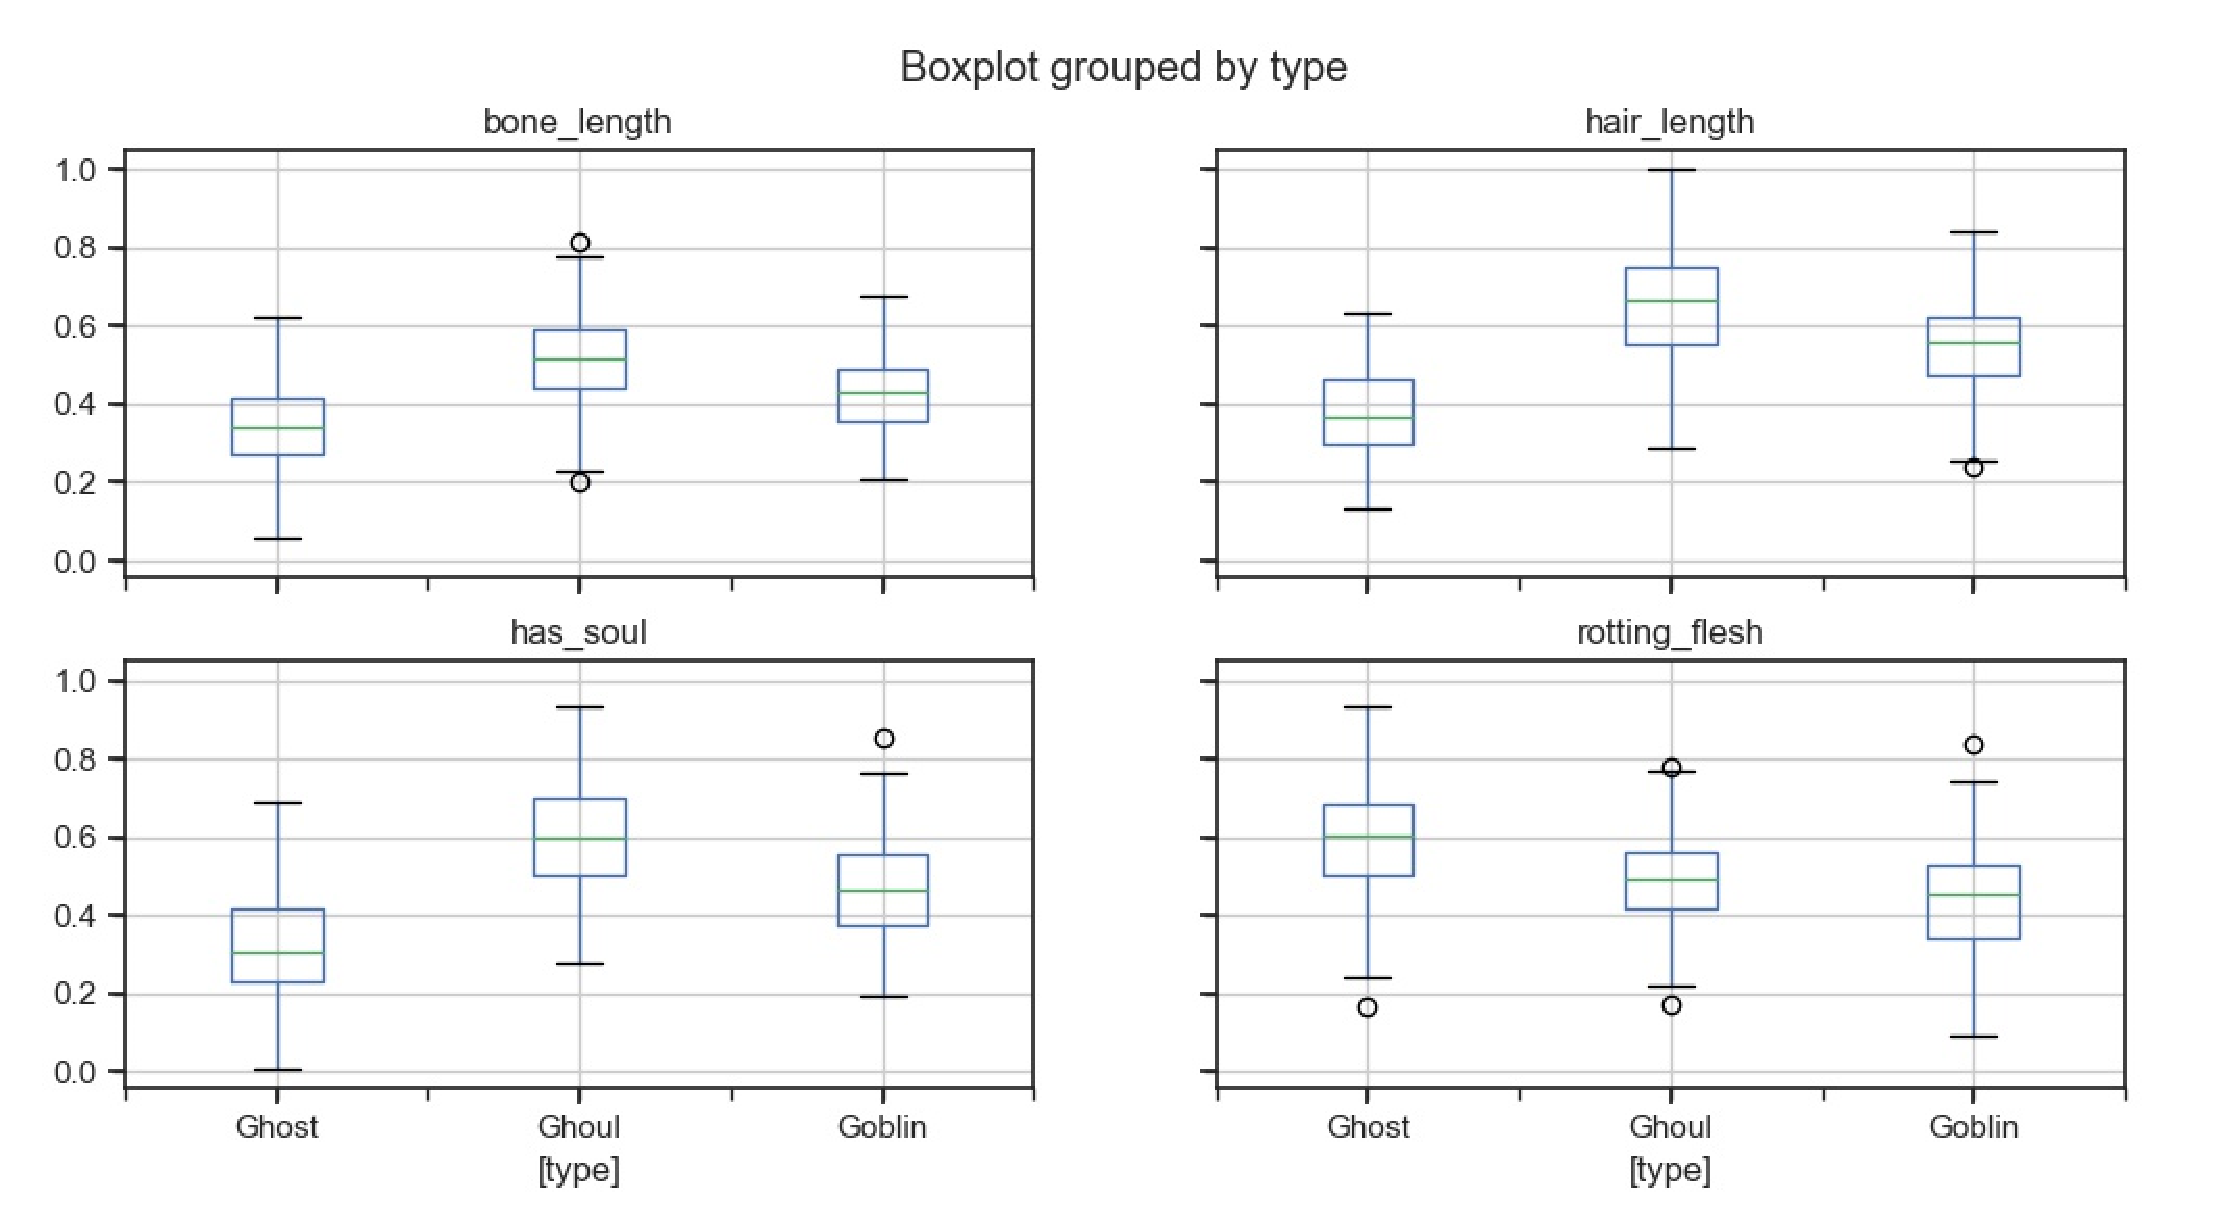
\includegraphics[scale=0.3]{figures/boxplot.eps}
	\caption{Boxplot Grouped by Type}
\end{figure}


\subsubsection{Pairwise Plot} 


Pairwise plot is 
a favorite in exploratory analysis 
to understand the relationship 
between all possible pairs 
of numeric variables. 
This pairplot ~\cref{fig:feature_scatterplot} 
shows that data is distributed normally. 
And while most pairs are widely scattered 
(in relationship to the type), 
some of them show clusters: 
hair_length and has_soul, 
hair_length and bone_length. 
So it may need to reassemble the data.

\begin{figure}[htbp]
	\centering
	\label{fig:feature_scatterplot}
	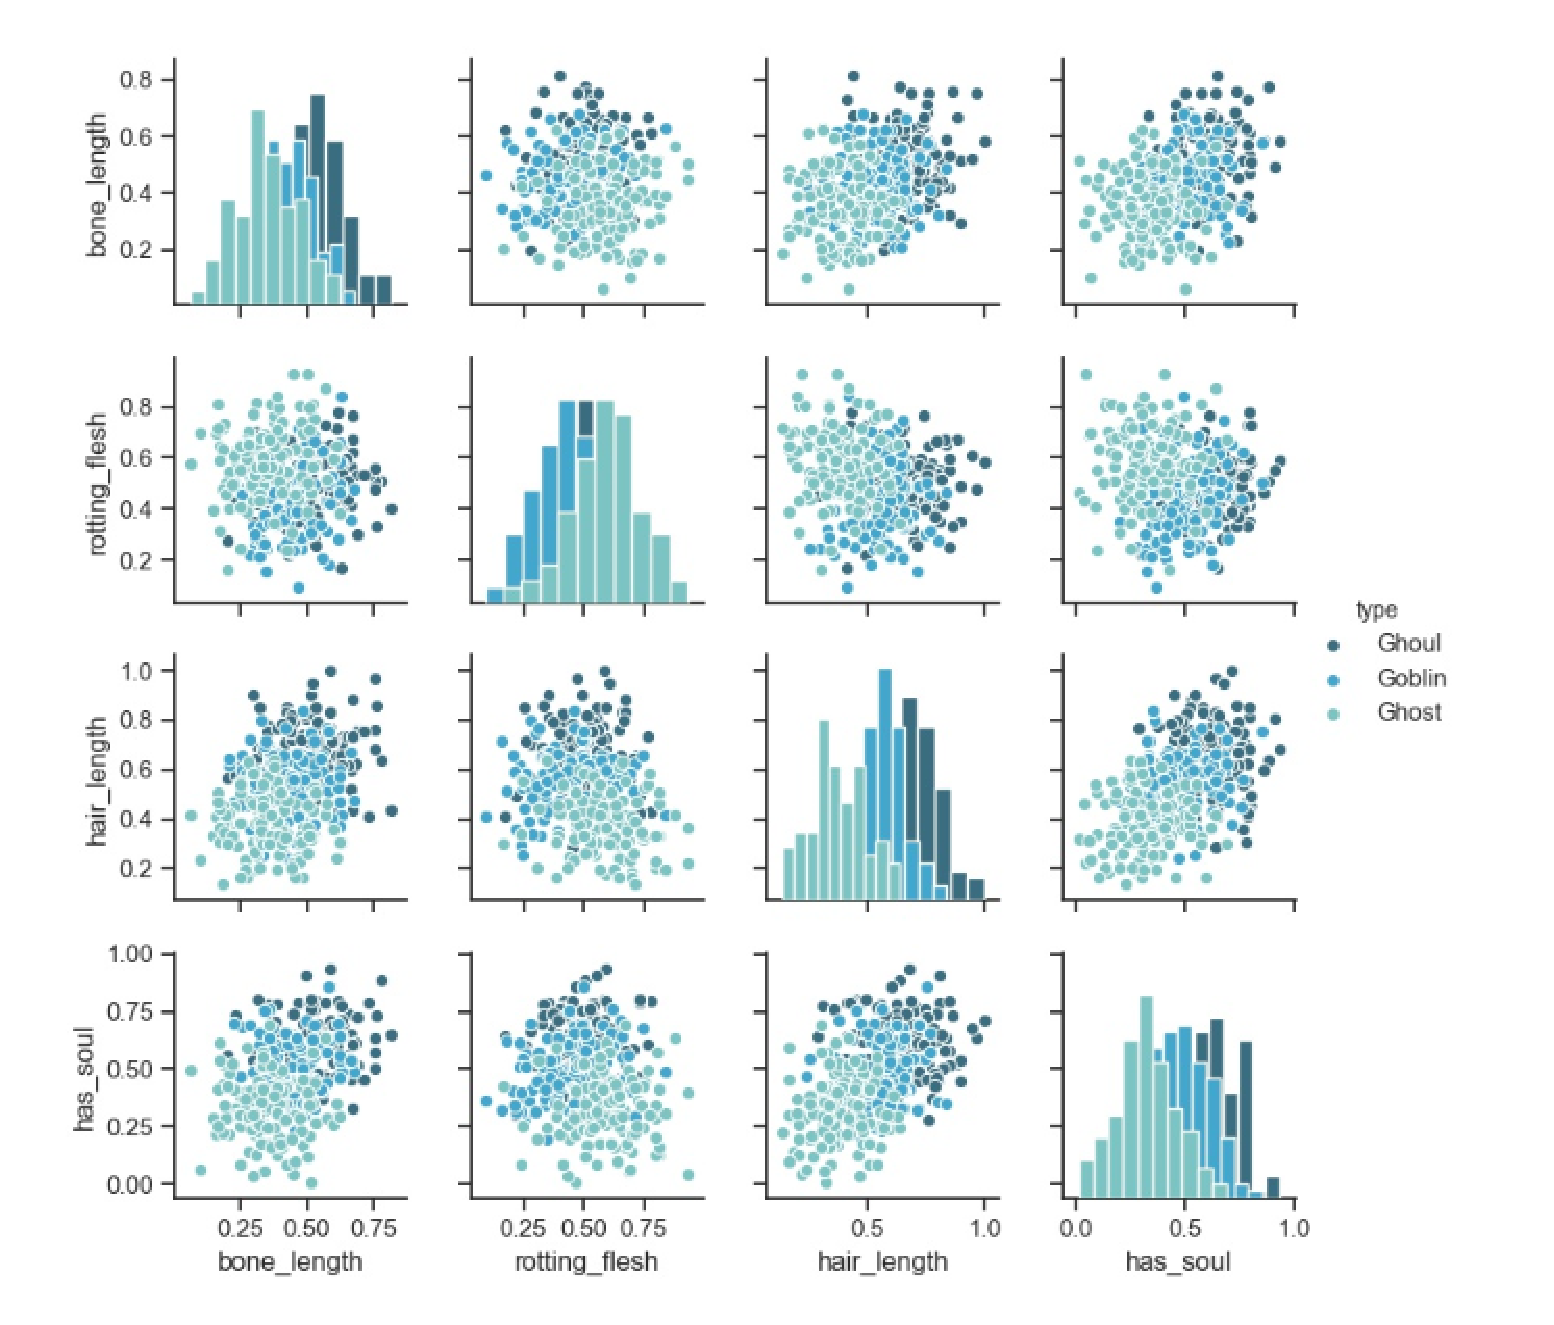
\includegraphics[scale=0.3]{figures/pairplot.eps}
	\caption{Feature Scatterplot}
\end{figure}


\subsubsection{Correllogram}


Correlogram is used to 
visually see the correlation metric 
between all possible pairs of numeric variables 
in a given dataframe. 
This figure ~\cref{fig:corr} 
help us to analyze features 
and their impact on the 'type' column. 
As we can see the 'type' column 
has a high value of negative correlation 
with columns 'has_soul' and 'rotting_flesh'. 
Although the correlation 
with the 'hair_length' is not very big.
There is no obvious linear relationship 
between variables

\begin{figure}[htbp]
	\centering
	\label{fig:corr}
	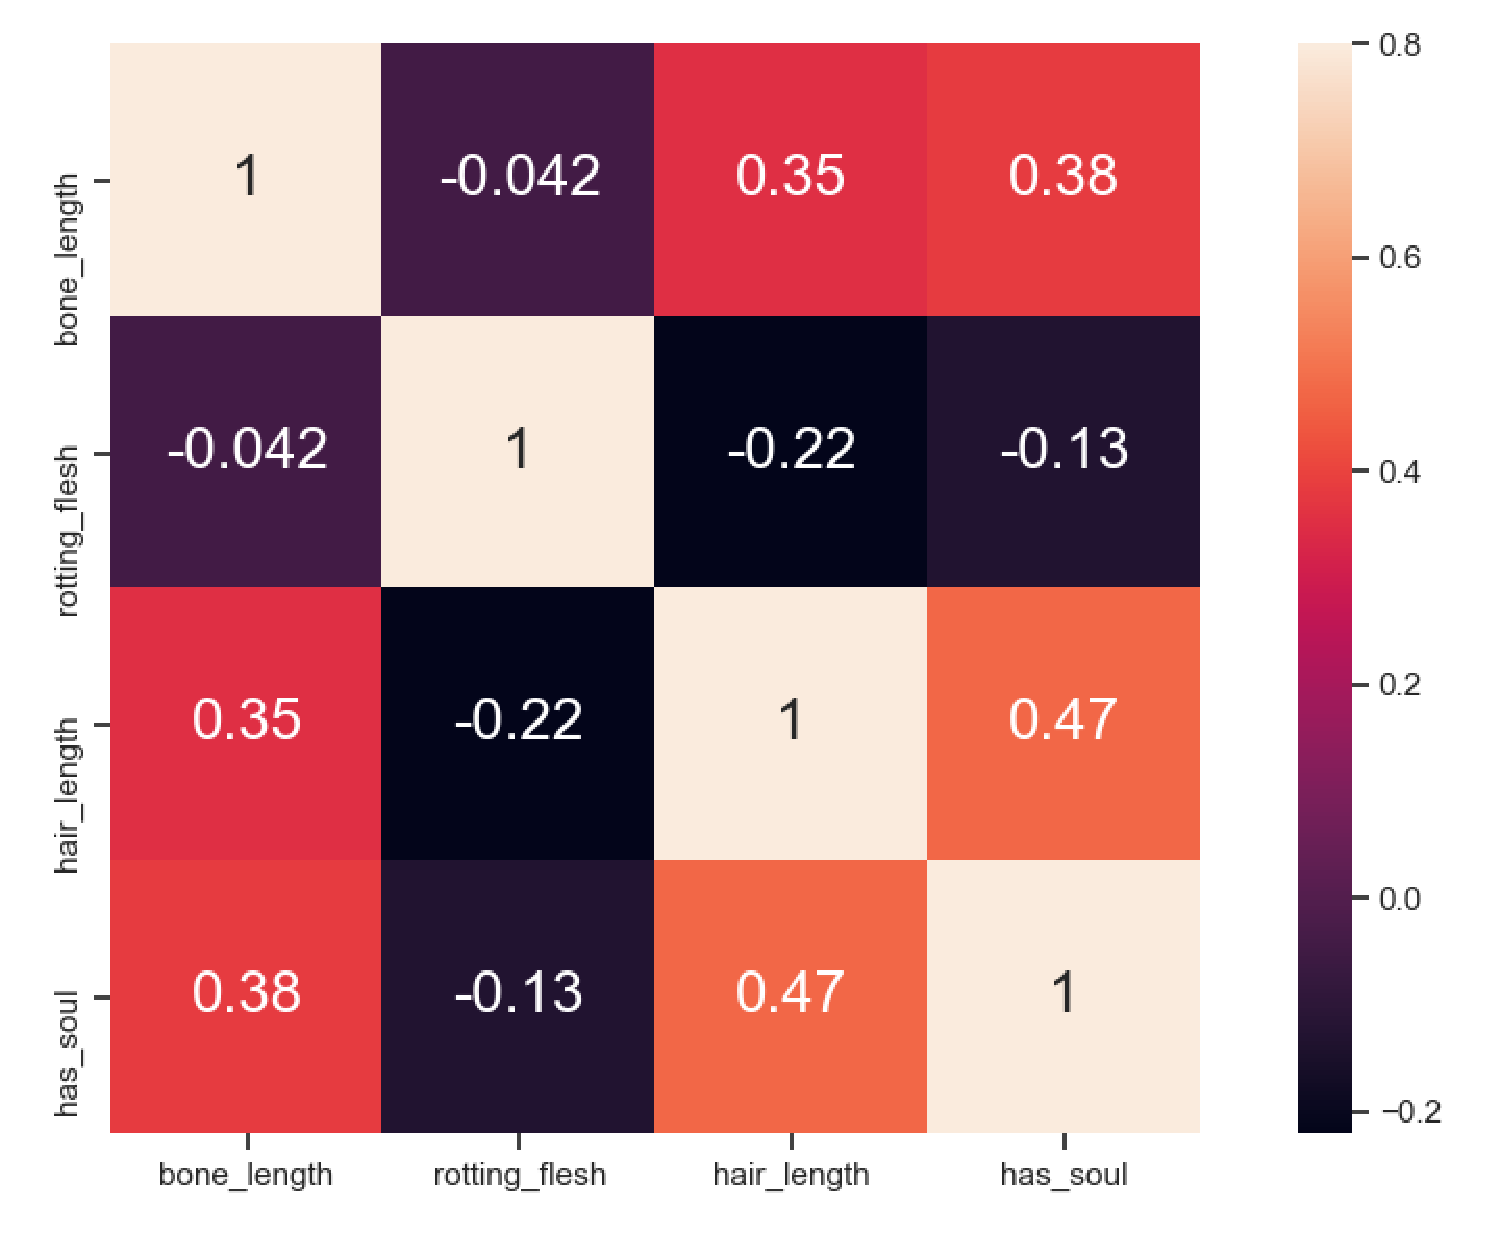
\includegraphics[scale=0.3]{figures/corr.eps}
	\caption{Correllogram}
\end{figure}


\subsubsection{Other Figures}


The following pictures 
are independent of 
the choice of algorithm. 
Because they look great, 
so I want to share with you.
%如果有时间的话,把这三张图片放在一排,然后稍微介绍一下

\begin{figure}[h]\centering
	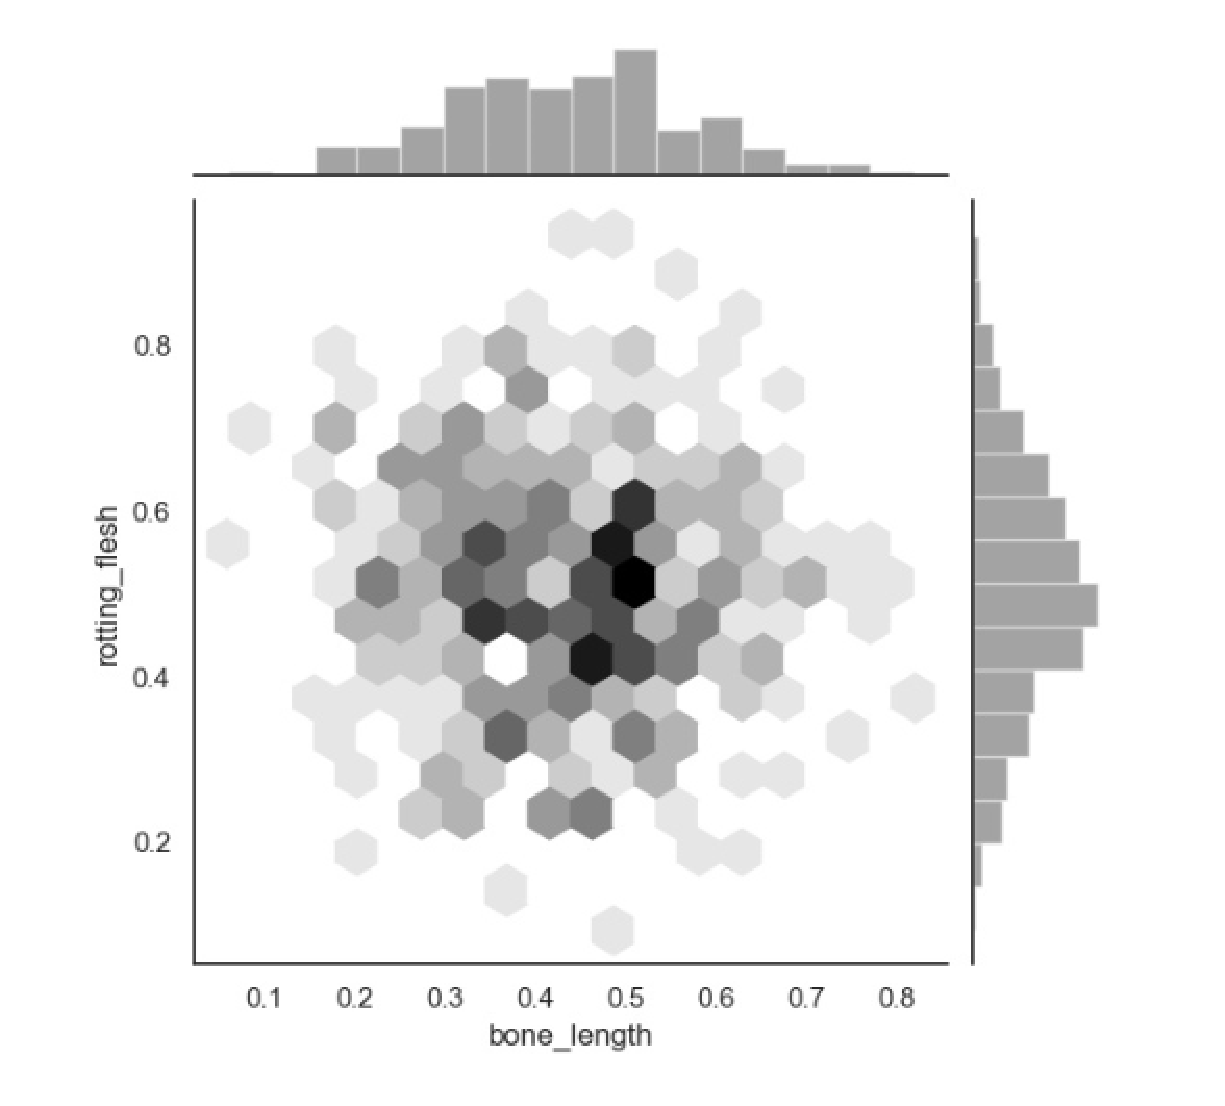
\includegraphics[scale=0.3]{figures/MHis.eps}
	\caption{Marginal Histogram}
\end{figure}

\begin{figure}[h]\centering
	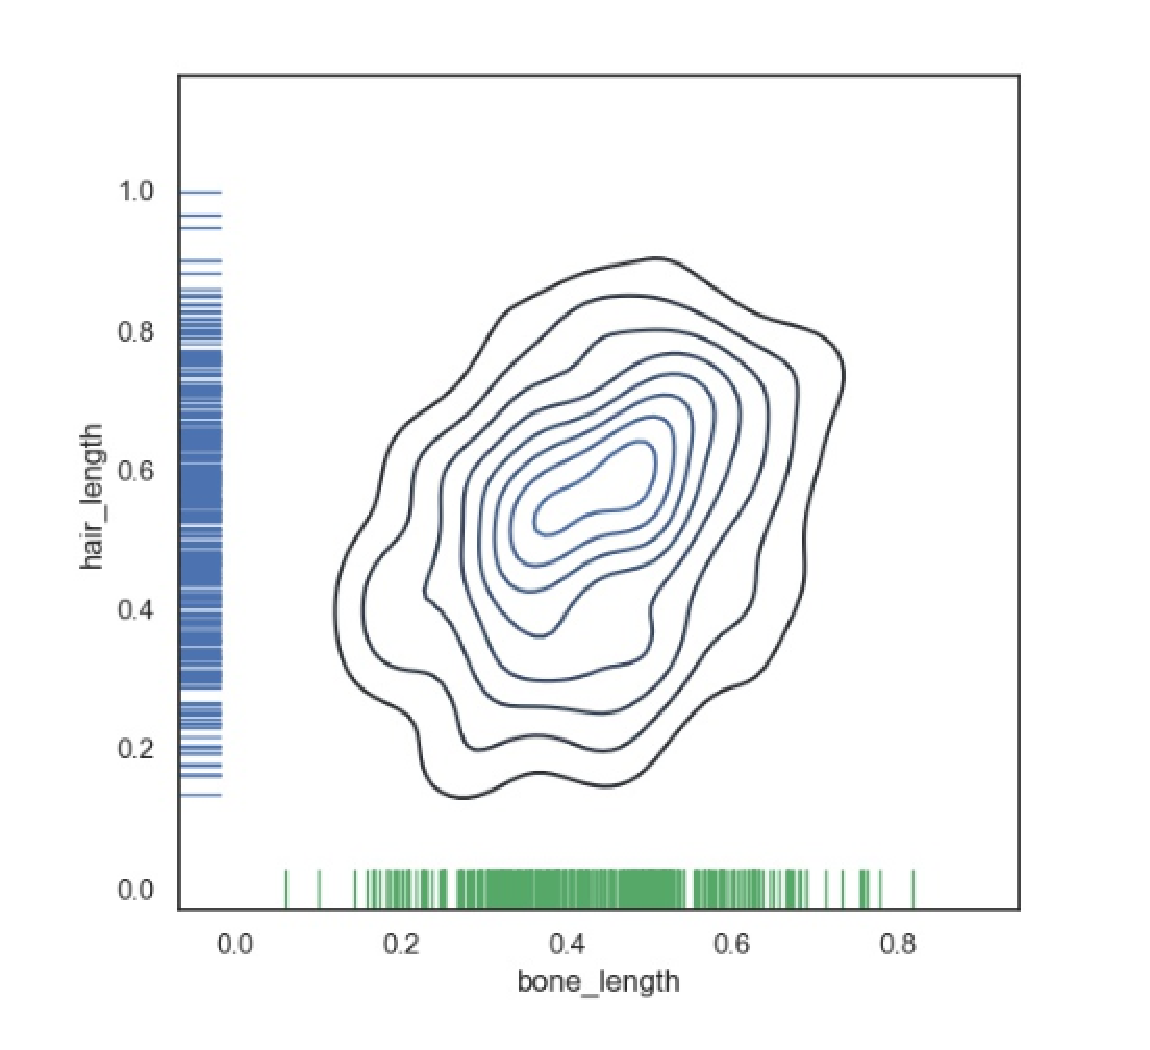
\includegraphics[scale=0.3]{figures/BDF.eps}
	\caption{Binary Density Function}
\end{figure}

\begin{figure}[h]\centering
	%\graphicspath{{figures/}{mine/}}
	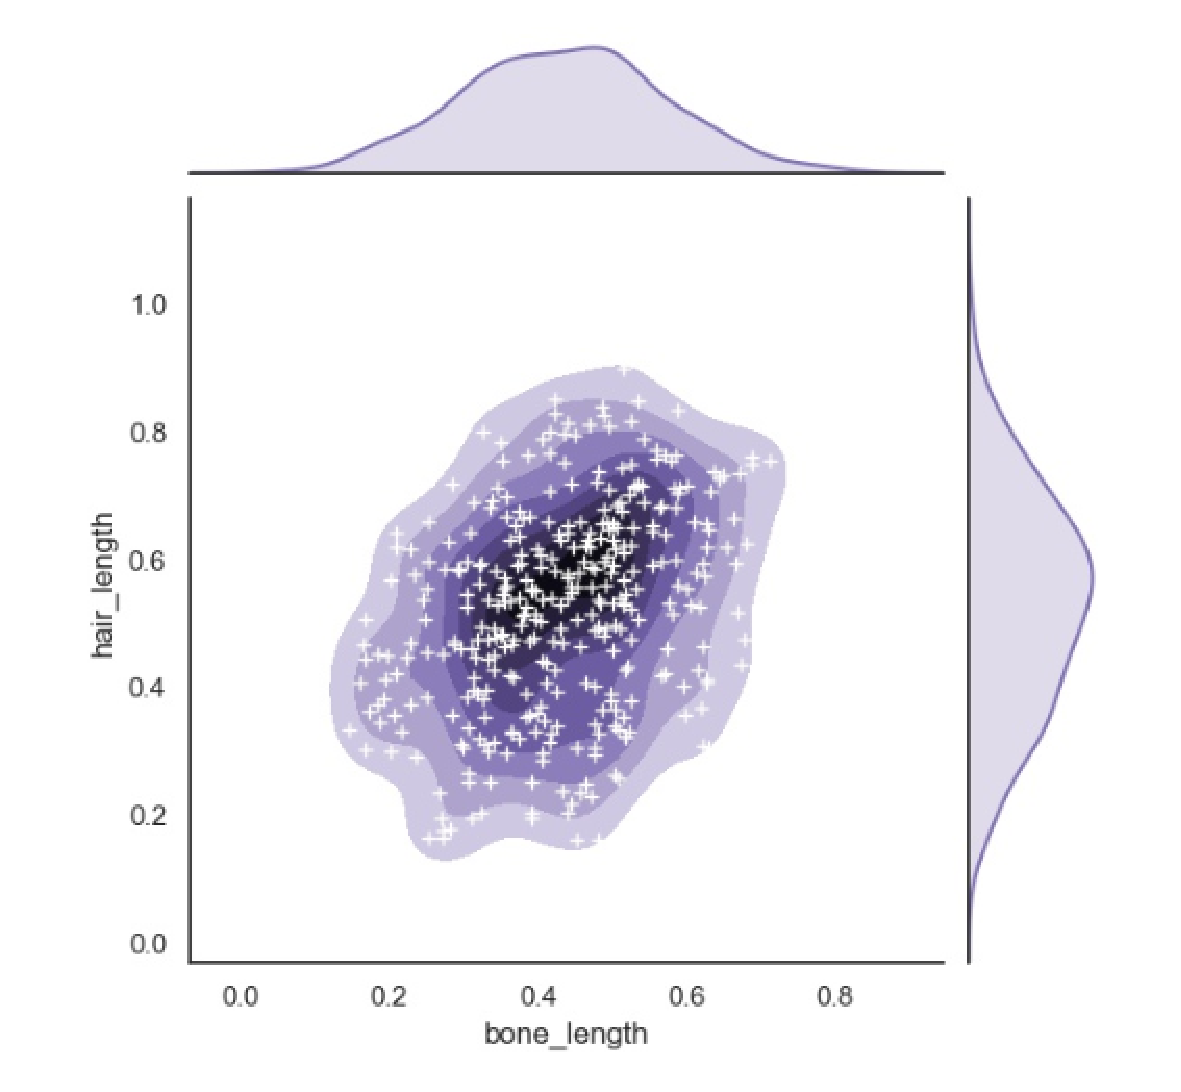
\includegraphics[scale=0.3]{figures/MBDF.eps}
	\caption{Marginal Binary Density Function}
\end{figure}


\subsection{Data Preparation}

\subsubsection{Great New Features}


As it can be seen from 
the pictures above 
the data is distributed normally. 
But some of them show clusters: 
hair_length and has_soul, 
hair_length and bone_length. 
So create new variables 
with multiplication of these columns: 

\begin{description}
	\item[hair_soul] row[’hair_length’]*row[’has_soul’] 
	\item[hair_bone]  row[hair_length]*row[bone_length] 
	\item[bone_soul]  row[bone_length]*row[has_soul] 
	\item[hair_soul_bone]  row[hair_length]*row[has_soul]*row[bone_length] 
\end{description}


Then analyse the new features in a pairplot, 
showing the picture ~\cref{fig:new_pairplot}
below. 
It can be seen from the picture that 
there is a clear linear relationship 
between the variables. 


\begin{figure}[htbp]\centering
	\label{fig:new_pairplot}
	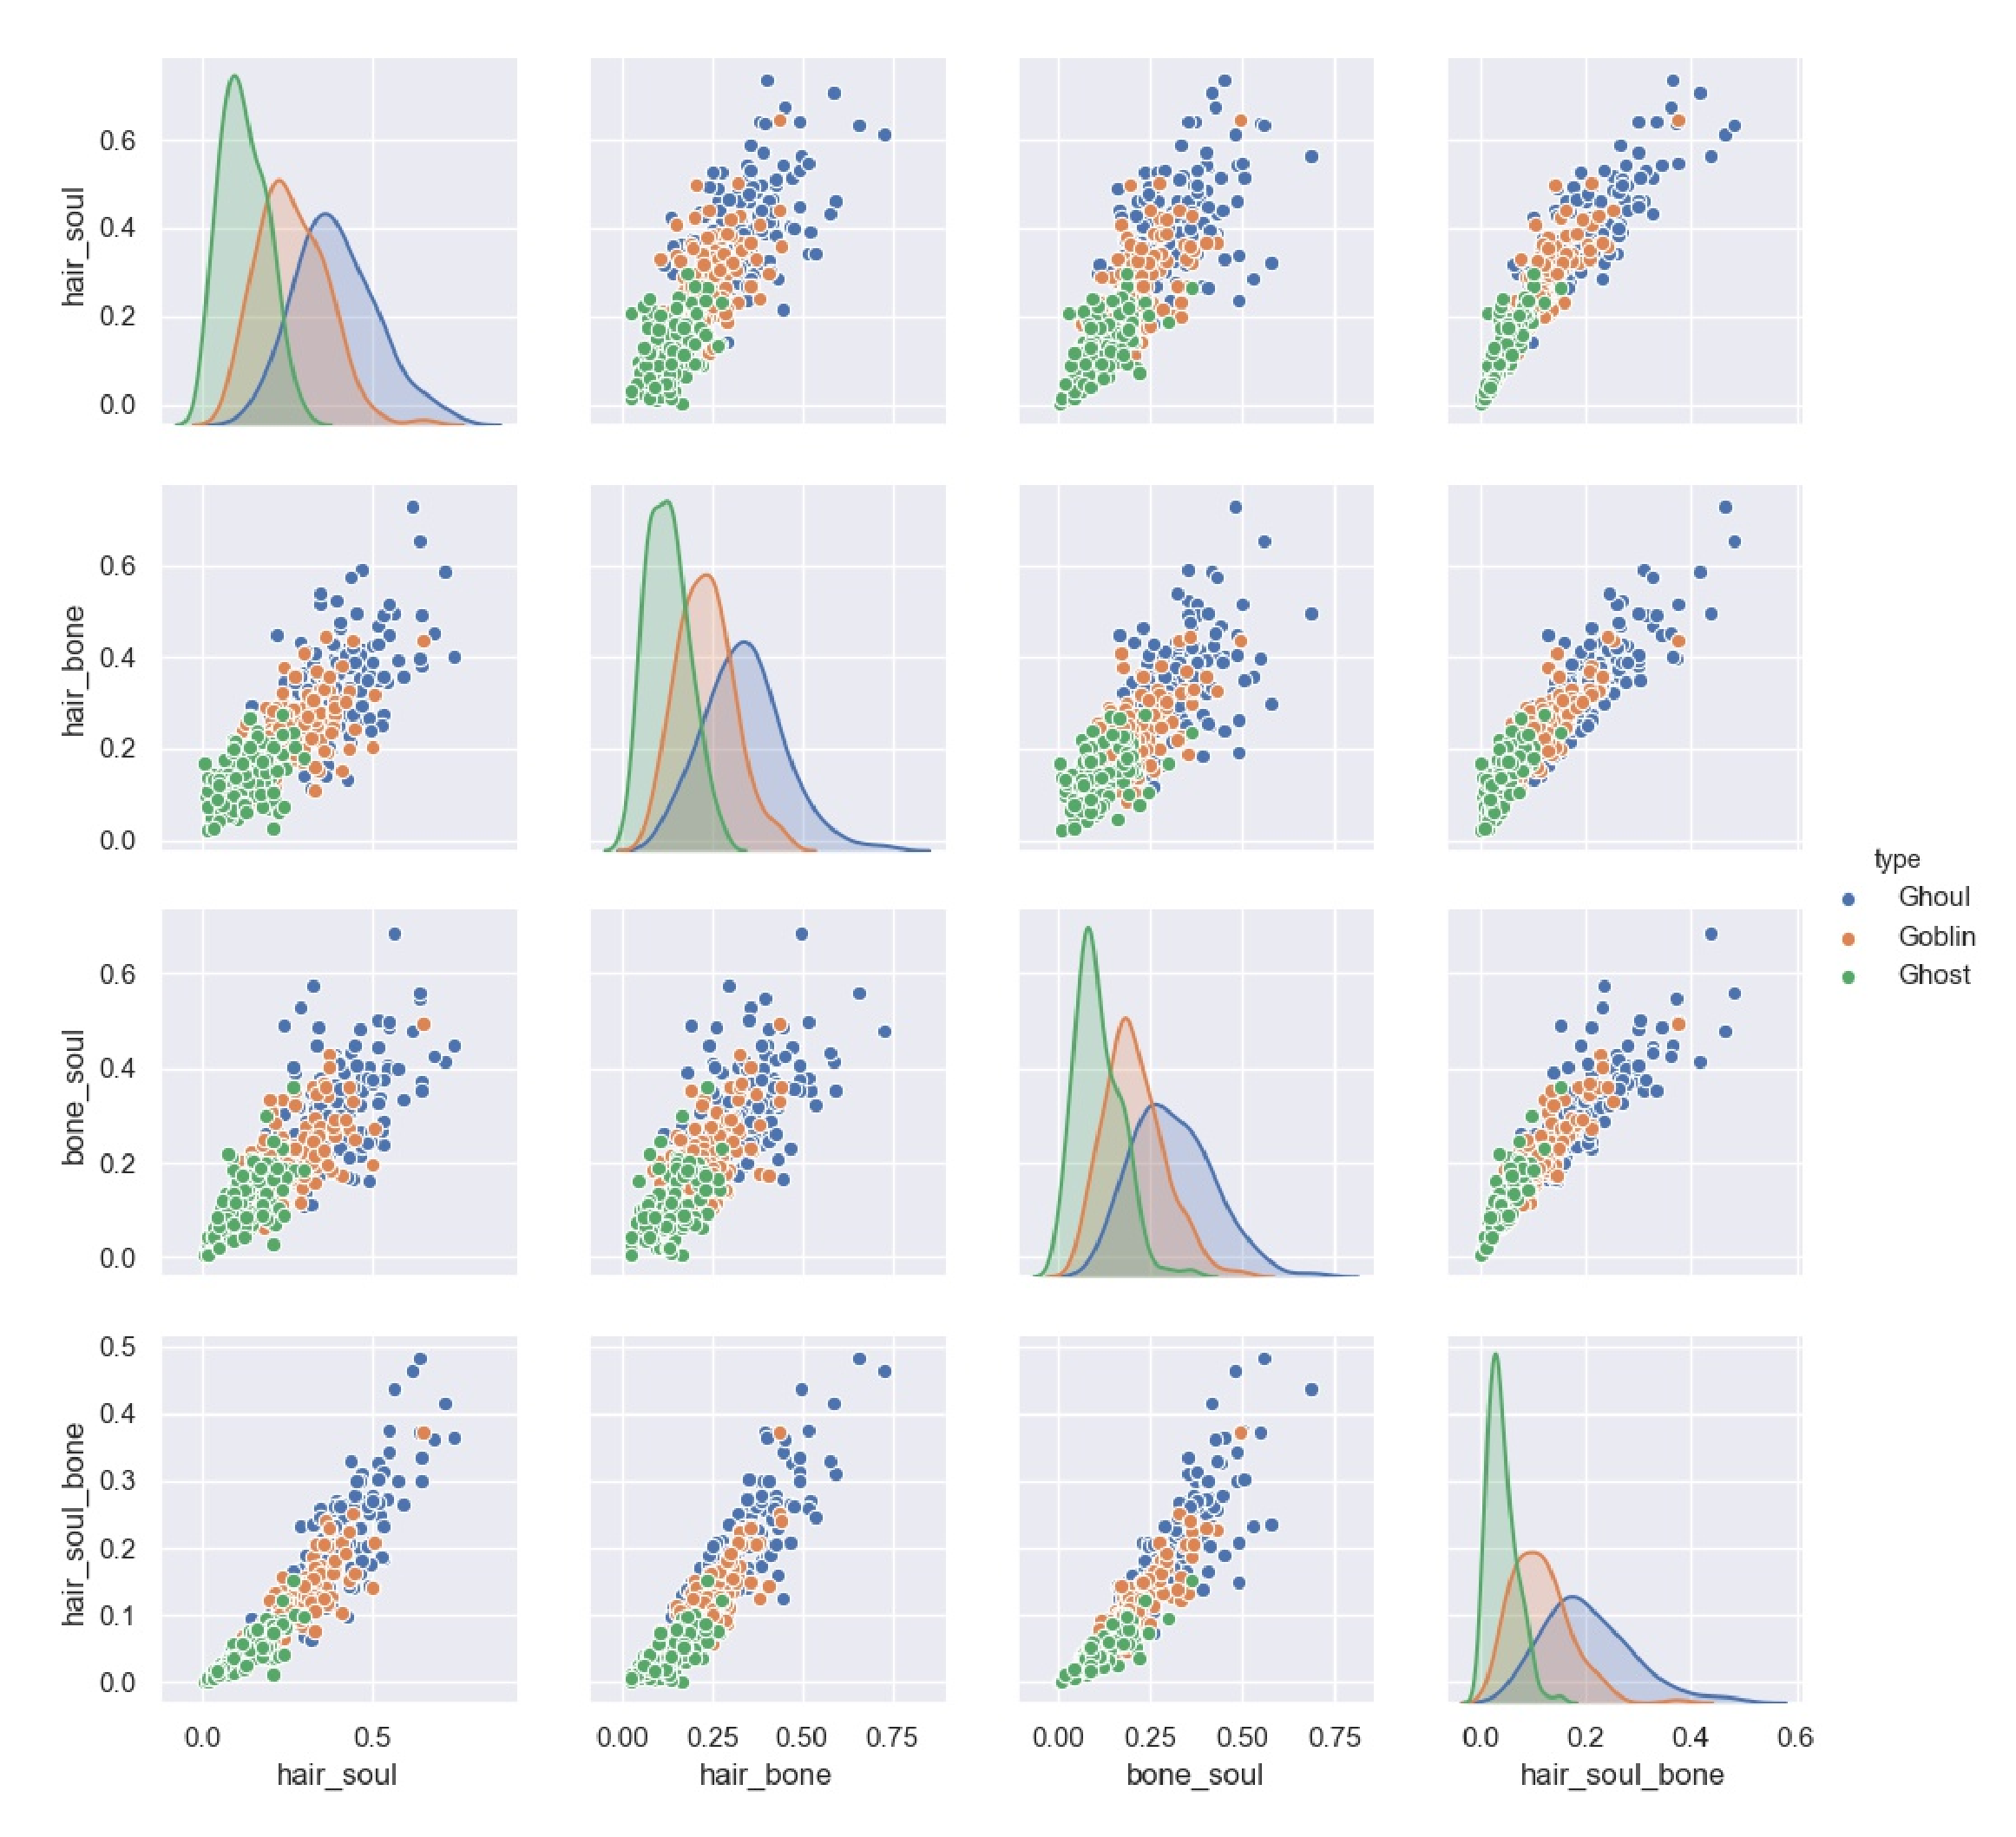
\includegraphics[scale=0.3]{figures/hist_1.eps}
	\caption{New Features Pairplot}
\end{figure}


\subsubsection{Feature Selection}


Train Random Forest model first, then using the Feature Importance this function to select the most important features. The following figure is a histogram ordered by feature importance. 


\begin{figure}[h]\centering
	%\graphicspath{{figures/}{mine/}}
	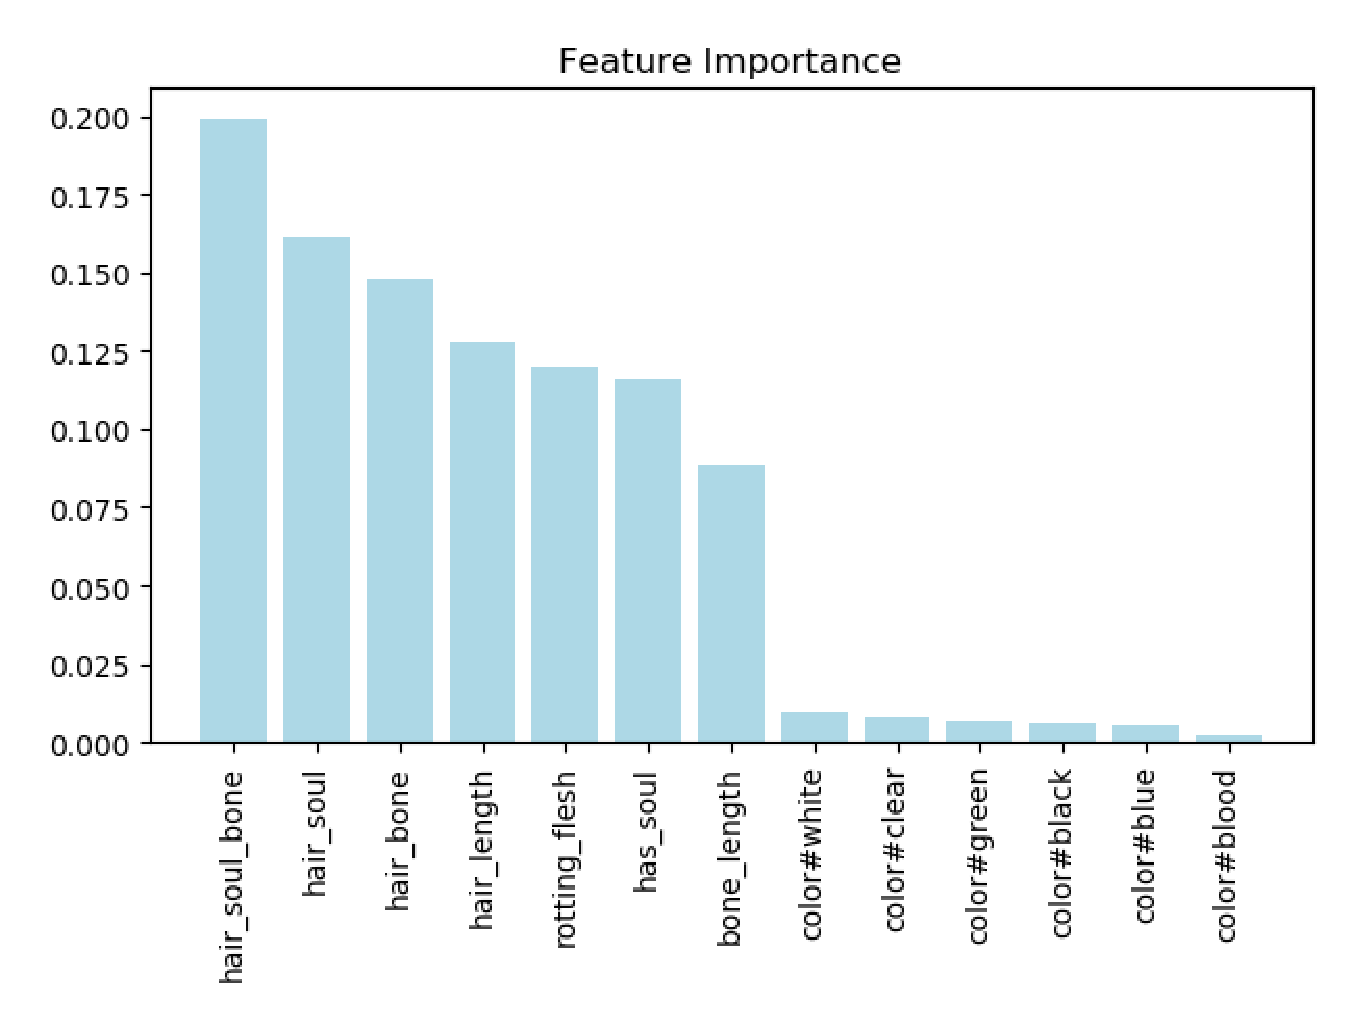
\includegraphics[scale=0.3]{figures/FEATURE.eps}
	\caption{Feature Importance}
\end{figure}


\section{Method}

\subsection{Ensemble Model}
There are many machine learning algorithms, 
select the following machine learning algorithms as Ensemble Model’s base models. 

\begin{itemize}
	\item RandomForestClassifier
	\item BaggingClassifier
	\item GradientBoostingClassifier
	\item LogisticRegression
	\item SVC
	\item KNeighborsClassifier 
	\item XGBClassifier
\end{itemize}

\subsection{Model Training}
meters,but the more important ones are generally not too many. Determine a set of optimal parameters through Grid Search. Because the training data is relatively small, a ten-fold cross-validation is used. %

\subsection{Neural Network}
There are three targets, 
use pandas.get_dummies this funtion to implement one-hot encoding of the tpyes.
The network contains forward, 
softmax and backpropagaation.


\section{Experiment and Result}

\subsection{Ensemble Model Training Result}

The results of using Grid Search to find the optimal parameters and the best accuracy of the algorithm are as 
 
follows. The best score is the score which is best in ten-fold cross-validation, best parameters is the 

parameters of the algorithms that can gain the best score, and the accuracy score is the accuracy of the 

algorithms on the test data. 

\subsubsection[Train_Data_1]{Use the all attribute value}

\begin{itemize}
	\item Best Parameters of the Base Models
	
	\begin{itemize}
		\item RandomForestClassifier
		
		\begin{description}
			\item[Best Parameters] 'criterion': 'entropy', 'max_depth': 5, 'max_features': None, 'n_estimators': 100
		\end{description}
		
		\item BaggingClassifier
		
		\begin{description}
			\item[Best Parameters] 'max_samples': 10, 'n_estimators': 100 'n_estimators': 100
		\end{description}
		
		\item GradientBoostingClassifier
		
		\begin{description}
			\item[Best Parameters] 'learning_rate': 0.3, 'max_depth': 2, 'n_estimators': 20
		\end{description}
		
		\item LogisticRegression
		
		\begin{description}
			\item[Best Parameters] 'C': 1, 'penalty': 'l1'
		\end{description}
		
		\item SVC
		
		\begin{description}
			\item[Best Parameters] 'C': 10, 'degree': 3, 'kernel': 'linear'
		\end{description}
		
		\item KNeighborsClassifier
		
		\begin{description}
			\item[Best Parameters] 'algorithm': 'auto', 'leaf_size': 10, 'n_neighbors': 20, 'p': 5, 'weights': 'uniform'
		\end{description}
		
	\end{itemize}
		
	
	\item Best Score of the Base Models
	
	\begin{table}[h]  \centering
		\caption{Best Score of the Base Models}
		\label{tbl:best_score}
		\begin{tabular}{ccccccc}
			\hline
			% after \\: \hline or \cline{col1-col2} \cline{col3-col4} ...
			Base Models& RandomForest & Bagging & Boosting & LogisticRegression & SVC & KNN \\
			\hline
			Best Score & 0.7143 & 0.7305 & 0.7358 & 0.7332 & 0.7385 & 0.7088 \\
			\hline 
			%\bottomrule
		\end{tabular}
	\end{table}
		
	
	\item Metrics Classification Report of Ensemble Model
	
	\begin{table}[h]  \centering
		\caption{Metrics Classification Report of Ensemble Model}
		\label{tbl:metrics_classification_ensemble}
		\begin{tabular}{ccccc}
			\hline
			& precision  &  recall & f1-score &  support\\
			\hline
			Ghost   &    0.80   &   0.83  & 0.82 & 24\\
			Ghoul  &  0.88  &  0.79  &   0.84   &   29\\
			Goblin  &   0.67  &  0.73 &  0.70  &   22\\
			\hline
			micro avg  &  0.79  &  0.79  & 0.79    &  75\\
			macro avg  &  0.78  & 0.78  &  0.78  &  75\\
			weighted avg  &   0.79  &  0.79 &  0.79  &  75\\
			\hline 
			%\bottomrule
		\end{tabular}
	\end{table}
	
	
\end{itemize}


\begin{itemize}
	\item RandomForestClassifier
	
	\begin{description}
		\item[Best Score] 0.7142857142857143
		\item[Best Parameters] 'criterion': 'entropy', 'max_depth': 5, 'max_features': None, 'n_estimators': 100
		\item[Accuracy Score] 0.8133333333333334
	\end{description}
	
	\item BaggingClassifier
	
	\begin{description}
		\item[Best Score] 0.7304582210242587
		\item[Best Parameters] 'max_samples': 10, 'n_estimators': 100 'n_estimators': 100
		\item[Accuracy Score] 0.68
	\end{description}
	
	\item GradientBoostingClassifier
	
	\begin{description}
		\item[Best Score] 0.7358490566037735
		\item[Best Parameters] 'learning_rate': 0.3, 'max_depth': 2, 'n_estimators': 20
		\item[Accuracy Score] 0.88
	\end{description}
	
	\item LogisticRegression
	
	\begin{description}
		\item[Best Score] 0.7331536388140162
		\item[Best Parameters] 'C': 1, 'penalty': 'l1'
		\item[Accuracy Score] 0.76
	\end{description}
	
	\item SVC
	
	\begin{description}
		\item[Best Score] 0.738544474393531
		\item[Best Parameters] 'C': 10, 'degree': 3, 'kernel': 'linear'
		\item[Accuracy Score] 0.7466666666666667
	\end{description}
	
	\item KNeighborsClassifier
	
	\begin{description}
		\item[Best Score] 0.7088948787061995
		\item[Best Parameters] 'algorithm': 'auto', 'leaf_size': 10, 'n_neighbors': 20, 'p': 5, 'weights': 'uniform'
		\item[Accuracy Score] 0.7333333333333333
	\end{description}
	%\item XGBClassifier
\end{itemize}
 




%\lstset{language=python}         
%\begin{lstlisting}[frame=single]  % Start your code-block
%rf = RandomForestClassifier(random_state = 0)
%clf = GridSearchCV(rf, param_grid = params, scoring = accuracy_scorer, cv = 10, n_jobs = -1)
%clf.fit(X_train, y_train)
%y_pred = clf.predict(X_test)
%\end{lstlisting}



Parallel Coordinates 
Parallel coordinates helps to visualize if a feature helps to segregate the groups effectively. If a segregation is effected, that feature is likely going to be very useful in predicting that group.
%Analyzing the correlation between other features it's possible to see that 'has_soul' and 'hair_length' have an interesting value as well as the column 'has_soul' with 'rotting_flesh'. Lets then try to extract some new features from here. 
%Test citation~\cite{BL12J01}. 
%\begin{JournalOnly}
%and~\citep{BJL11J01} or~\citet{BJL11J01}.
%\end{JournalOnly}

%This is for~\cref{tbl:overall-experiments}, 
%\todo[fancyline]{Testing.}
%and this is for~\cref{sec-conclusions}.
%\todo[noline]{A note with no line back to the text.}%
%\gangli{This is comment from Gang.}
%\qwu{Response from QW}

Number:
\num{123}.
\numlist{10;30;50;70},
\numrange{10}{30},
\SIlist{10;30;45}{\metre},
and
\SI{10}{\percent}

\missingfigure[figcolor=white]{Testing figcolor}


\begin{ConferenceOnly}
We have \SI{10}{\hertz},
\si{\kilogram\metre\per\second},
the range: \SIrange{10}{100}{\hertz}.
$\nicefrac[]{1}{2}$.

\missingfigure{Make a sketch of the structure of a trebuchet.}

\end{ConferenceOnly}


For~\cref{eq:test},
as shown below:

\begin{equation}\label{eq:test}
a = b \times \sqrt{ab}
\end{equation}

\blindmathpaper

\section{Preliminaries} \label{sec-preliminaries}

\blindtext

\gliMarker  %TODO: GLi Here


\section{Method} \label{sec-method}

\blindtext
\blindlist{itemize}[3]
\blinditemize
\blindenumerate

\blindmathtrue
\blindmathfalse
\blinddescription


\section{Experiment and Analysis} \label{sec-experiment}


\begin{table}  \centering
  \caption{Precision Comparison on Event Detection Methods}
  \label{tbl:overall-experiments}
  \begin{tabular}{cccc}
\toprule
    % after \\: \hline or \cline{col1-col2} \cline{col3-col4} ...
    & OR Event Detection & AC Event Detection & TC Event Detection \\
\midrule
    precision & 0.83 & 0.69 & 0.46 \\
    recall & 0.68 & 0.48 & 0.36 \\
    F-score & 0.747 & 0.57 & 0.4 \\
\bottomrule
\end{tabular}
\end{table}


\section{Conclusions} \label{sec-conclusions}

\blindtext

\section*{Acknowledgment}

\lipsum[1]


The authors would like to thank \ldots

